%%%%%%%%%%%%%%%%%%%%%%%%%%%%%% -*- Mode: Latex -*- %%%%%%%%%%%%%%%%%%%%%%%%%%%%
%% 09-01.tex --     Automated Software Engineering submission
%% Author          : Philip Johnson 
%% Created On      : Tue Jan 06 10:41:51 2009
%% Last Modified By: Philip Johnson
%% Last Modified On: Wed Jan 14 11:58:50 2009
%%%%%%%%%%%%%%%%%%%%%%%%%%%%%%%%%%%%%%%%%%%%%%%%%%%%%%%%%%%%%%%%%%%%%%%%%%%%%%%
%%   Copyright (C) 2009  Philip Johnson
%%%%%%%%%%%%%%%%%%%%%%%%%%%%%%%%%%%%%%%%%%%%%%%%%%%%%%%%%%%%%%%%%%%%%%%%%%%%%%%
%% 

\documentclass[smallextended]{svjour3}     % onecolumn (second format)
\usepackage{graphicx}
\usepackage{natbib}
\usepackage{url}             
\journalname{Automated Software Engineering}

\begin{document}
\title{Operational Definition and Automated Inference of Test-Driven Development with Zorro}
\author{Hongbing Kou \and Philip M. Johnson}
\institute{Hongbing Kou and Philip M. Johnson \at 
           Collaborative Software Development Laboratory  \\
           Department of Information and Computer Sciences \\
           University of Hawaii \\
           Honolulu, HI 96822 \\
           Tel.: 808-956-3489\\
           Fax:  808-956-3548\\
           \email{hongbing@hawaii.edu} \\
           \email{johnson@hawaii.edu} \\
}

\date{Received: date / Accepted: date}

\maketitle

\begin{abstract}

Test-driven development (TDD) is a style of development named for its most
visible characteristic: the design and implementation of test cases prior
to the implementation of the code required to make them pass. Many claims
have been made for TDD: that it can improve implementation as well as
design quality, that it can improve productivity, that it results in 100\%
coverage, and so forth.  However, research to validate these claims has
yielded mixed and sometimes contradictory results.  We believe that at
least part of the reason for these results stems from differing
interpretations of the TDD development style, along with an inability to
determine whether programmers actually follow whatever definition of
TDD is in use.

Zorro is a system designed to automatically determine whether a developer
is complying with an operational definition of Test-Driven Development
(TDD) practices.  Automated recognition of TDD can benefit the software
development community in a variety of ways, from inquiry into the ``true
nature'' of TDD, to pedagogical aids to support the practice of test-driven
development, to support for more rigorous empirical studies on the
effectiveness of TDD in both laboratory and real world settings.

This paper describes the Zorro system, its operational definition of TDD,
the analyses made possible by Zorro, and three empirical evaluations of the
system.


\keywords{Test Driven Design \and Hackystat }
\end{abstract}

\section{Introduction}
\label{intro}

Substantial claims have been made regarding the effectiveness of
test-driven development (TDD). Evangelists claim that it naturally
generates 100\% coverage, improves refactoring, provides useful executable
documentation, produces higher code quality, and reduces defect rates
\citep{Beck:03}.  Unfortunately, the empirical research results have been
equivocal.  Some results are positive: \cite{Bhat:06} found that
introducing TDD at Microsoft decreased defect rates significantly in two
projects, and \cite{Maximilien:03} transitioned an IBM development team to
TDD with a 50\% improvement in quality. But other results are negative:
\cite{Muller:02} found that TDD resulted in less reliable software than the
control group and \cite{Erdogmus:05} found that TDD software was of no
higher quality than the control group.

Why might the research results on TDD be so mixed?  We believe that part of
the reason stems from two methodological issues that impede both progress
on understanding TDD's current effectiveness and future improvements to the
technique. 

First, TDD is often defined in a relatively simplistic and ambiguous manner
using toy examples.  This can mislead developers into thinking that TDD
does not apply to their more complex development situations. It can also
lead to different organizations defining the practice of TDD in very
different ways.

Second, research on TDD suffers from the ``process compliance problem''.
In other words, the experimental designs do not have mechanisms in place to
verify that subjects who are supposed to be using TDD practices are,
indeed, using them.  The lack of control over process compliance in these
experiments means that differences in outcomes may be due, at least in
part, to variance in understanding what it means to do TDD, as opposed to
differences between the control and experimental groups.

To address these problems, we believe that the software research and
development community needs to agree upon at least one (if not more)
standard, operational definitions of TDD. Furthermore, these definition(s)
must allow for a practical way to assess compliance in both laboratory and
real-world settings.

In this paper, we present Zorro, a system for automated recognition of TDD
practices.  In essence, Zorro gathers a stream of low-level developer
behaviors (such as invoking a unit test, editing production code, invoking
a refactoring operation) while programming in an IDE, partitions this event
stream into a sequence of development ``episodes'', then applies a
rule-based system to determine whether or not each episode constitutes an
instance of a TDD practice according to the operational definition encoded in the rules.

Zorro illustrates one approach to addressing the issues mentioned above
that hinder the research and practice of TDD today.  Automatic collection
and analysis of data makes Zorro practical for use in both laboratory and
real-world settings: once installed, there is no overhead on the developer
with respect to data collection.  Second, Zorro can be used to develop a
variety of operational definitions of TDD. A Zorro ``TDD definition''
consists of the set of developer behaviors that must be collected, the
manner in which this timestamped stream of events are partitioned into
episodes, and the rules used to determine if an episode is TDD.  By
providing a way to define an operational definition of TDD, Zorro addresses
the compliance problem by enabling researchers and practitioners to
precisely characterize the extent to which the given definition of TDD was
applied (or not) in any given development scenario.  Furthermore, Zorro's
episode-based approach to TDD recognition provides a more nuanced approach
to characterizing the use of TDD by developers: rather than a binary,
``all-or-nothing'' approach, Zorro enables TDD usage characterizations
based on percentages, such as ``Developer A used TDD 73\% of the time''.

Zorro has undergone initial empirical evaluation through classroom and
industry-based case studies.  These results indicate that Zorro is a viable
approach to automated TDD recognition.

This paper is organized as follows.  Section \ref{sec:RelatedWork} presents
work related to Zorro.  (Reference other sections here).

\section{Related Work}
\label{sec:RelatedWork}

\subsection{The practice of TDD}

Test-Driven Development \citep{Beck:03} is a software development 
best practice popularized by Extreme Programming \citep{Jeffries:00,Beck:00}. 
It is normally introduced as a very simple practice consisting of only two rules:

\begin{enumerate}
\item Write new code only if an automated test has failed.
\item Eliminate duplication.
\end{enumerate} 

An equally simple but more process-oriented description is the the 
``stop light'' metaphor \citep{Beck:03}: 
\begin{enumerate}
\item Red - Write a little test that does not work, and perhaps does not even compile at first.
\item Green - Make the test work quickly, committing whatever sins are necessary in the process.
\item Yellow (Refactor) - Eliminate all the duplication created by merely getting the test to work.
\end{enumerate}

Important characteristics of TDD practice, according to \citep{Beck:01,Beck:03},  include the following.

{\em Write the test first.}
This is the key characteristic of TDD. If you are using 
TDD, you should ``never write a line of functional 
code without a broken test case''

{\em Short iterations.}
Quickly adding functional code to make test pass is important
to TDD. An iteration should last a few seconds to 
several minutes only. If hours of work are needed to make a 
test pass, then this is a sign that the developer should have divided the programming 
task into smaller subtasks that could be solved in a shorter
period of time.

{\em Frequent refactoring.}
Code is consistently refactored in TDD to create the simplest
possible design. The existence of a suite of unit tests gives 
developers the ``courage'' to refactor the code

{\em Rapid feedback.}
Unit testing is usually supported by the XUnit
framework that is now available for most languages.
After new functional code is added, developers should invoke
the unit tests to test it right away. This feedback should be available
within seconds or minutes. 

{\em One ball in the air at a time.}  In typical software development, the
developer tries to simultaneously balance several requirements, including
system structure design, algorithm choice, code efficiency, readability,
communication with other code, and so forth.  Martin Fowler is quoted as
describing that process as being like ``keeping several balls in the air at
once''.  In contrast, it is claimed that in TDD, the developer only keeps
``one ball in the air at once'' and concentrates only on that ball. For
example, in the development step, the developer only needs to make the test
pass without worrying about whether it is a good or bad design. In the
refactoring step, the developer only worries about what makes a good
design.

{\em The code should always work.} 
In TDD, developers should run 
all tests at the end of each iteration. If any test has failed, 
the developer should fix it right away. The fix should be easy because 
only a small amount of code is written in each iteration. If running 
all tests after an iteration is not feasible, the continuous 
integration can be set up to run them all once a day or several 
times a day. 

TDD advocates claim that adherence to this approach can simultaneously
improve both quality and productivity \citep{Beck:01,Janzen:05}.  Because
software quality is hard to measure, TDD practitioners and researchers
often use code coverage as a proxy for software quality. The code developed
in TDD should be 100\% covered since no functional code is created without
a corresponding unit test.

The claimed rationale for why TDD improves productivity is a bit more
complicated. Functional code and test code are both products. Testing is
part of the design process, and it does not take a long time to write a
small test. If developers need to write same amount of test code, TDD
should save development time because less time is spent on tests than in
the traditional test last or ad-hoc development methods. In addition, TDD
users claim that the method reduces the overall amount of time spent on
debugging, with a resulting increase in overall
productivity \citep{Williams:03}.

\subsection{Empirical evaluation of TDD}
\label{sec:related-empirical}

Much research work has been conducted on studying important outcomes of TDD
such as software quality and developer productivity in recent years. In
addition to anecdotal experience reports
\citep{George:04,Maximilien:03,Williams:03,Kaufmann:03,Edwards:04,Bhat:06},
researchers have run controlled experiments
\citep{Muller:02,Matjaz:03,Erdogmus:05} to compare TDD against other
development methods such as test last and ad hoc. We categorize the
research as ``academic'' or ``industrial'' depending upon whether the test
subjects are students or professional developers.

\subsubsection{Empirical Evaluation in Academic Settings}

\cite{Muller:02} conducted a study in an XP class in
Germany to test TDD against traditional programming.  The acceptance tests
were provided to both the TDD group and the control group. Interestingly,
students in the TDD group spent more time but their programs were less
reliable than the control group.

\cite{Edwards:04} adopted TDD in a junior-level class to compare
whether students got more reliable code after the use of TDD and WEB-CAT,
an assignment submission system. It turned out that the students using TDD
reduced their defect rate dramatically (45\% fewer defects/KSLOC using a
proxy metric) after adopting TDD, and a posttest survey found that TDD
students were more confident of the correctness and robustness of their
programs.

Similarly, \cite{Kaufmann:03} conducted a pilot study
on implications of TDD in an advanced project-oriented software engineering
course. They also reported that TDD helped to improve software quality and
programmers' confidence.

\cite{Matjaz:03} designed a controlled experiment to compare TDD with
Iterative Test-Last approach (ITL), which is a slightly modified TDD
development process in the order of ``code-test-refactor''.  This study
found that TDD is somewhat different from ITL but the difference is very
small.

A more recent study on the effectiveness of TDD 
\citep{Erdogmus:05} used the well-defined test-last
and TDD approaches as in \cite{Matjaz:03}. This study
concluded that TDD programmers wrote more tests per unit of programming
effort. More test code tends to increase software quality. Thus, TDD
appears to improve the quality of software but TDD group in the study did
not achieve better quality on average than test-last group.

\subsubsection{Empirical Evaluation in Industrial Settings}
Several attempts have been made by researchers to study software quality
and developer productivity improvements of TDD in industrial settings.  

\cite{George:04} ran a set of structured experiments
with 24 professional pair programmers in three companies. Each pair was
randomly assigned to a TDD group or a control group to develop a bowling
game application. The final projects were assessed at the end of the
experiment.  They found that TDD practice appears to yield code with
superior external code quality as measured by a set of blackbox test cases,
and TDD group passed 18\% more test cases. However, the TDD group spent
16\% more time on development, which could have indicated that achieving
higher quality requires some additional investment of time. Interestingly,
and in the contrast to the empirical findings, 78\% of the subjects
indicated that TDD practice would improve programmers' productivity.

\cite{Maximilien:03} transitioned a software team
from an ad-hoc approach to testing to TDD unit testing practice at IBM, and
this team improved software quality by 50\% as measured by Functional
Verification Tests (FVT).

\cite{Williams:03} conducted another case
study in IBM to study TDD. Compared to a baseline project developed in a 
traditional fashion, the defect density of the project developed 
in TDD was reduced by 40\% as measured by functional verification and 
regression tests. The productivity was not impacted by the additional 
focus on producing test code. 

\cite{Geras:04} isolated TDD from other XP
practices, and investigated the impact of TDD on developer productivity and
software quality. In their research, TDD does not require more time but
developers in TDD group wrote more tests and executed them more frequently,
which may have led to future time savings on debugging and development.

Another study of TDD at Microsoft conducted by Bhat and Nagappan
\citep{Bhat:06} reported remarkable software quality improvement as 
measured in number of defects per KLOC. After introduction of TDD, 
project A (Windows) reduced its defects rate by 2.6 times, and project 
B (MSN) reduced its defect rate by 4.2 times, compared to the organizational
average. Reportedly, developers in project A spent 35\% more development
time, and developers in project B spent 15\% more development time, than
the developers in non-TDD projects spent.

\subsection{A comparative analysis of the studies}

The research findings regarding the effect of TDD practices on software quality 
and developer productivity are mixed,  as shown in 
Tables \ref{tab:ControlledTDDResearch} (Controlled Studies) and \ref{tab:CaseStudyTDDResearch} (Case Studies). 
The study conducted at Microsoft \citep{Bhat:06} and the study conducted 
at the University of Karlsruhe \citep{Muller:02} are two extreme cases. In 
\cite{Bhat:06}, the developers improved software quality up to four 
times after adopting TDD. In comparison, the TDD group in \cite{Muller:02} 
yielded less reliable programs than the control group. 

\begin{table}[ht]
\caption{Controlled Empirical Experiments on TDD}
\begin{tabular}{|l|l|l|p{1.0in}|p{1.0in}|} \hline 
Investigator      & A/I & Subjs.	& Software Quality	& Developer Productivity \\ \hline
\cite{George:04}  & I & 24	& TDD passed 18\% more tests & 16\% more time \\ \hline
\cite{Geras:04}   & I & 14	& TDD had better quality & No impact \\ \hline 
\cite{Kaufmann:03}& A &  8 & N/A	    & 50\% improvement \\ \hline
\cite{Erdogmus:05}& A & 35	& No change	  & Improved productivity \\ \hline
\cite{Muller:02}  & A & 19 & Less reliable, but better reuse	& No change \\ \hline
\cite{Matjaz:03}  & A & 38	& No change	  & No change \\ \hline
\end{tabular}
\label{tab:ControlledTDDResearch}
\end{table}

\begin{table}[ht]
\caption{Empirical Case Studies on TDD}
\begin{tabular}{|l|l|l|p{1.0in}|p{1.0in}|} \hline 
Investigator        & A/I      & Subjs.	& Software Quality	& Developer Productivity \\ \hline
\cite{Maximilien:03}& I &  9	& 50\% reduction in defect density	& Minimal impact \\ \hline
\cite{Williams:03}  & I & 9	& 40\% reduction in defect density	& No change \\ \hline
\cite{Bhat:06}      & A & 11	& 2-4 times reduction in defect density	& 35\% and 15\% more time \\  \hline
\cite{Edwards:04}   & A & 59	& 54\% fewer defects	& N/A \\ \hline
\end{tabular}
\label{tab:CaseStudyTDDResearch}
\end{table}


\subsection{Automated Software Process Research}
\label{sec:related-automation}

Automated software process research systems are often top-down in nature:
they take a high-level description of a system process and use it to
constrain, control, or understand the actual development behaviors.
Process programming \citep{Sutton:95}, modeling \citep{Curtis:92} and
simulation \citep{Turnu:04,Jensen:05} are typical research methods for
studying software processes.  Process conformance, at least as performed by Zorro,
is a bottom-up process in which the actual development behaviors are
the input to, as opposed to the output from, the system.

Cook and Wolf \citep{Cook:95,Cook:96} developed a client-server system
named Balboa to automate the process discovery using finite state machine
(FSM). Balboa collects developers' invocations of Unix commands and CVS
commits to construct event streams. It then uses a neural network, a MARKOV
chain, and data mining algorithms to discover the FSM of software
processes. With Balboa, Cook and Wolf were able to reproduce the ISPW 6/7
process in their research.

\cite{Jensen:04,Jensen:05} simulated an automated approach to discover and
model the open source software development processes. They took advantage
of prior knowledge to discover the software development processes by
modeling the process fragments using a PML description. Their prototype
simulation found that they could detect unusually long activities and
problematic cycles of activities. They suggested that a bottom-up strategy,
together with a top-down process meta-modeling is suitable for automated
process discovery. 

For this research, we chose a rule-based system to study process
conformance of low-level software processes. Instead of asking process
experts to inspect the FSM of the executed process as Cook and Wolf did
\citep{Cook:95}, we converted the process knowledge into a set of rules and
used them to infer the software development behaviors. Our method is very
close to Jansen's and Scacchi's approach \citep{Jensen:04} except that we
used rules rather than PML for process descriptions.

\cite{Wang:04} argued that the empirical research of TDD suffers from the
construct validity problem (as is also the case in some other empirical
software engineering research) because it lacks process conformance. They
developed a prototype called ``TestFirstGauge'' to study the process
conformance of TDD by mining the in-process log data collected by
Hackystat.

TestFirstGauge aggregates software development data collected
by Hackystat to derive programming cycles of TDD. They used T/P ratio 
(lines of test code verse lines of production code), testing effort 
against production effort and cycle time distribution as the indicator 
of TDD process conformance. This project precedes the Zorro software 
system \citep{csdl2-06-02}, and in fact it stimulated our research interest 
in studying low-level software process conformance. Unlike the
prototype implementation of TestFirstGauge in VBA using an Excel
spreadsheet, Zorro is integrated into the Hackystat system for automation,
reuse, and flexibility using rule-based system \citep{Friedman-Hill:03}.

Similarly, \cite{Wege:04} also focused on automated support of TDD process
assessment, but his work has a limitation in that it uses the CVS history
of code. Developers typically do not commit on-going project data at the
granularity of seconds, minutes or hours, making this data collection
technique problematic for the purpose of TDD inference. At least for the
operational definition of TDD developed in this research, collecting rapid
low-level development activities is crucial to correctly identifying its
occurrence.

\section{Zorro}
\label{sec:zorro}

\subsection{Architectural components}

As illustrated in Figure \ref{fig:ZorroArchitecture}, the Zorro
architecture consists of three subsystems: (1) Hackystat, which collects
low-level developer behaviors; (2) SDSA (Software Development Stream
Analysis), a Hackystat application that supports generic analysis of
development event streams; and (3) Zorro, an SDSA application, which
defines the specific rules and analyses necessary for recognition and
interpretation of the TDD behavior of a developer.

\begin{figure*}[th]
  \center
  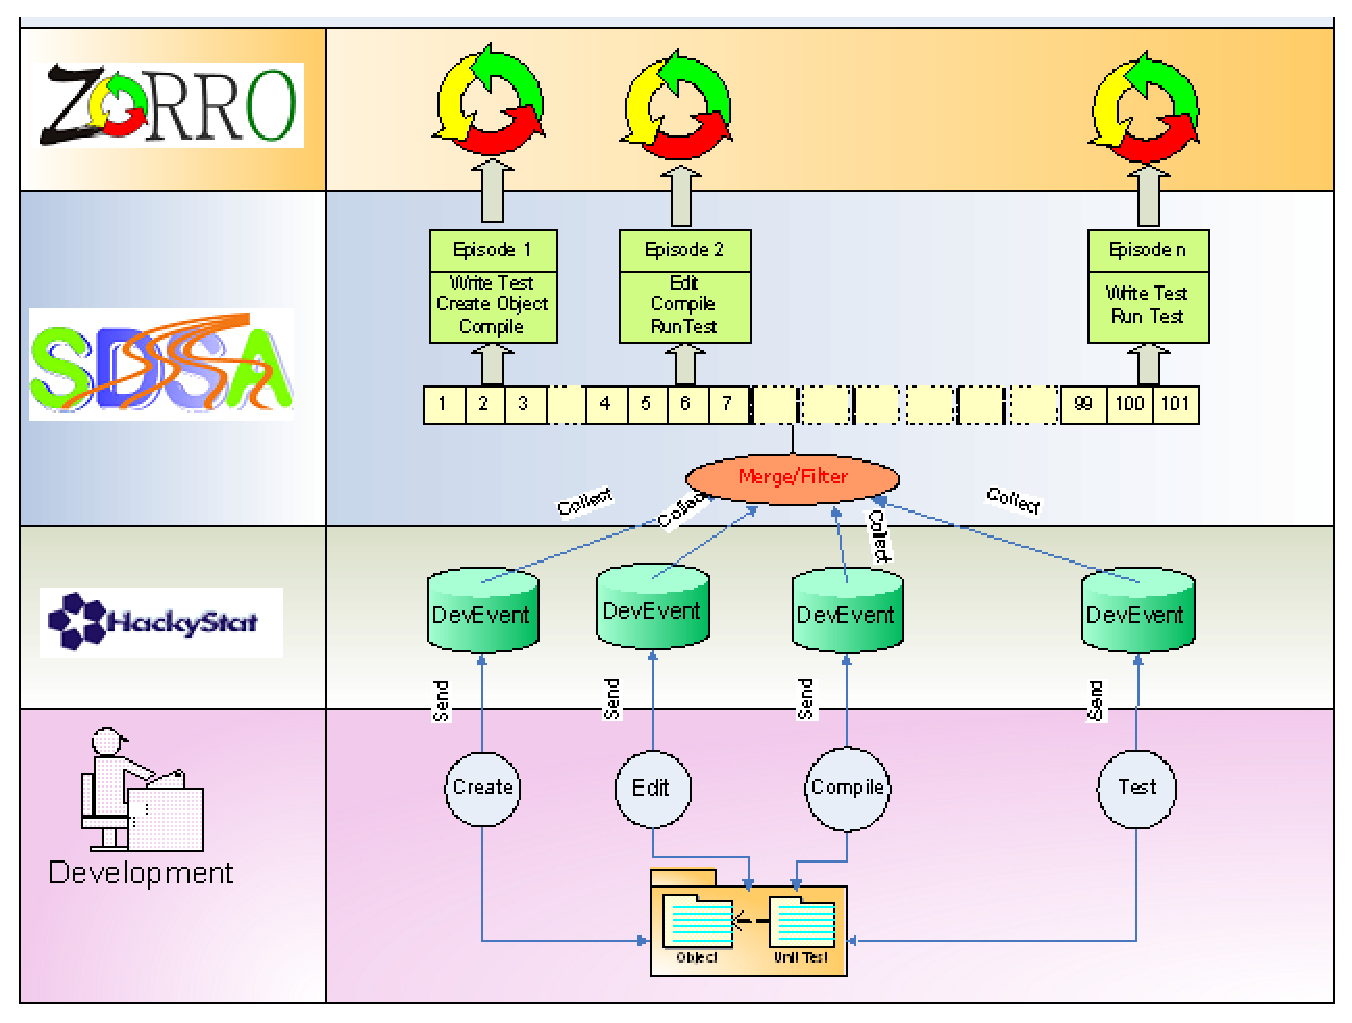
\includegraphics[width=1.0\textwidth]{zorro-architecture.eps}
  \caption{The Zorro Architecture}
  \label{fig:ZorroArchitecture}
\end{figure*} 


{\bf Hackystat.} Hackystat is an open source framework for automated
collection and analysis of software engineering process and product data
that we have been developing since 2001. Hackystat supports unobtrusive
data collection via specialized ``sensors'' that are attached to
development environment tools and that send structured ``sensor data type''
instances to a web-based Hackystat service for subsequent analysis.  Over
two dozen sensors are currently available, including sensors for IDEs
(Emacs, Eclipse, Vim, VisualStudio, Idea), configuration management (CVS,
Subversion), bug tracking (Jira, Bugzilla), testing and coverage (JUnit,
CppUnit, Emma, JBlanket), system builds and packaging (Ant), static
analysis (Checkstyle, PMD, FindBugs, LOCC, SCLC), and so forth.
Applications of the Hackystat Framework in addition to our work on SDSA and
Zorro include in-process project management \citep{csdl2-04-11}, high
performance computing \citep{csdl2-04-22}, and software engineering
education \citep{csdl2-03-12}.

Zorro requires the developer's IDE to be instrumented with a Hackystat
sensor that can collect at least the following kinds of events: unit test
invocations (and their results), compilation events (and their results),
refactoring events (such as renaming, moving), and editing (or code
production) events (such as whether the file has changed in state during
the previous 30 seconds, and what the resulting size of the file is in
statements, methods, and/or test case assertions).

We have implemented a Hackystat sensor for the Eclipse IDE to collect these
events for the Java language, and a Hackystat sensor for the Visual Studio
IDE to collect these events for the C\# language.


{\bf SDSA.} Software Development Stream Analysis (SDSA) is a Hackystat-based application that
provides a generic framework for organizing and analyzing the various kinds
of data received by Hackystat as input to a rule-based, time-series
analysis.

SDSA begins by merging the events collected by various sensors into a
single sequence, ordered by time-stamp, called the ``development stream''.
This is followed by a process called tokenizing, which results in a
sequence of higher-level ``episodes''.  These constitute the atomic
building blocks for whatever process is being recognized.  For any given
application of the SDSA framework, tokenization involving defining the
specific events to be combined to generate the development stream, as well
as the boundary condition that separates the final event in one episode
from the initial event in the next. For example, development events could
include things like a unit test invocation, a file compilation, a
configuration management commit, or a refactoring operation.  Example
boundary conditions could include a configuration management system
checkin, test pass event, or a buffer transition.

Once the development stream has been abstracted into a sequence of
episodes, the next step in SDSA is to classify each episode according to
whatever process is under analysis.  SDSA provides an interface to the JESS
rule-based system engine to enable developers to specify part or all of the
classification process as a set of rules.


{\bf Zorro.} The Zorro architectural layer provides extensions to Hackystat and SDSA
necessary for the automated recognition of Test Driven Development
behaviors.  Let's now examine Zorro's inferencing mechanism in more detail. 

\subsection{TDD Inference using Zorro: A simple example}

As introduced above, TDD inference in Zorro consists of the following
steps: (a) collection of low-level developer sensor data using Hackystat;
(b) abstraction of the sensor data into a developer event stream; (c)
partitioning of the event stream into episodes; and finally
(d) classification of the resulting episodes as either TDD-conformant or TDD
non-conformant.  Figure \ref{fig:SDSA-Example} illustrates an example of
the last three steps in this process.

\begin{figure}[htbp]
  \centering
  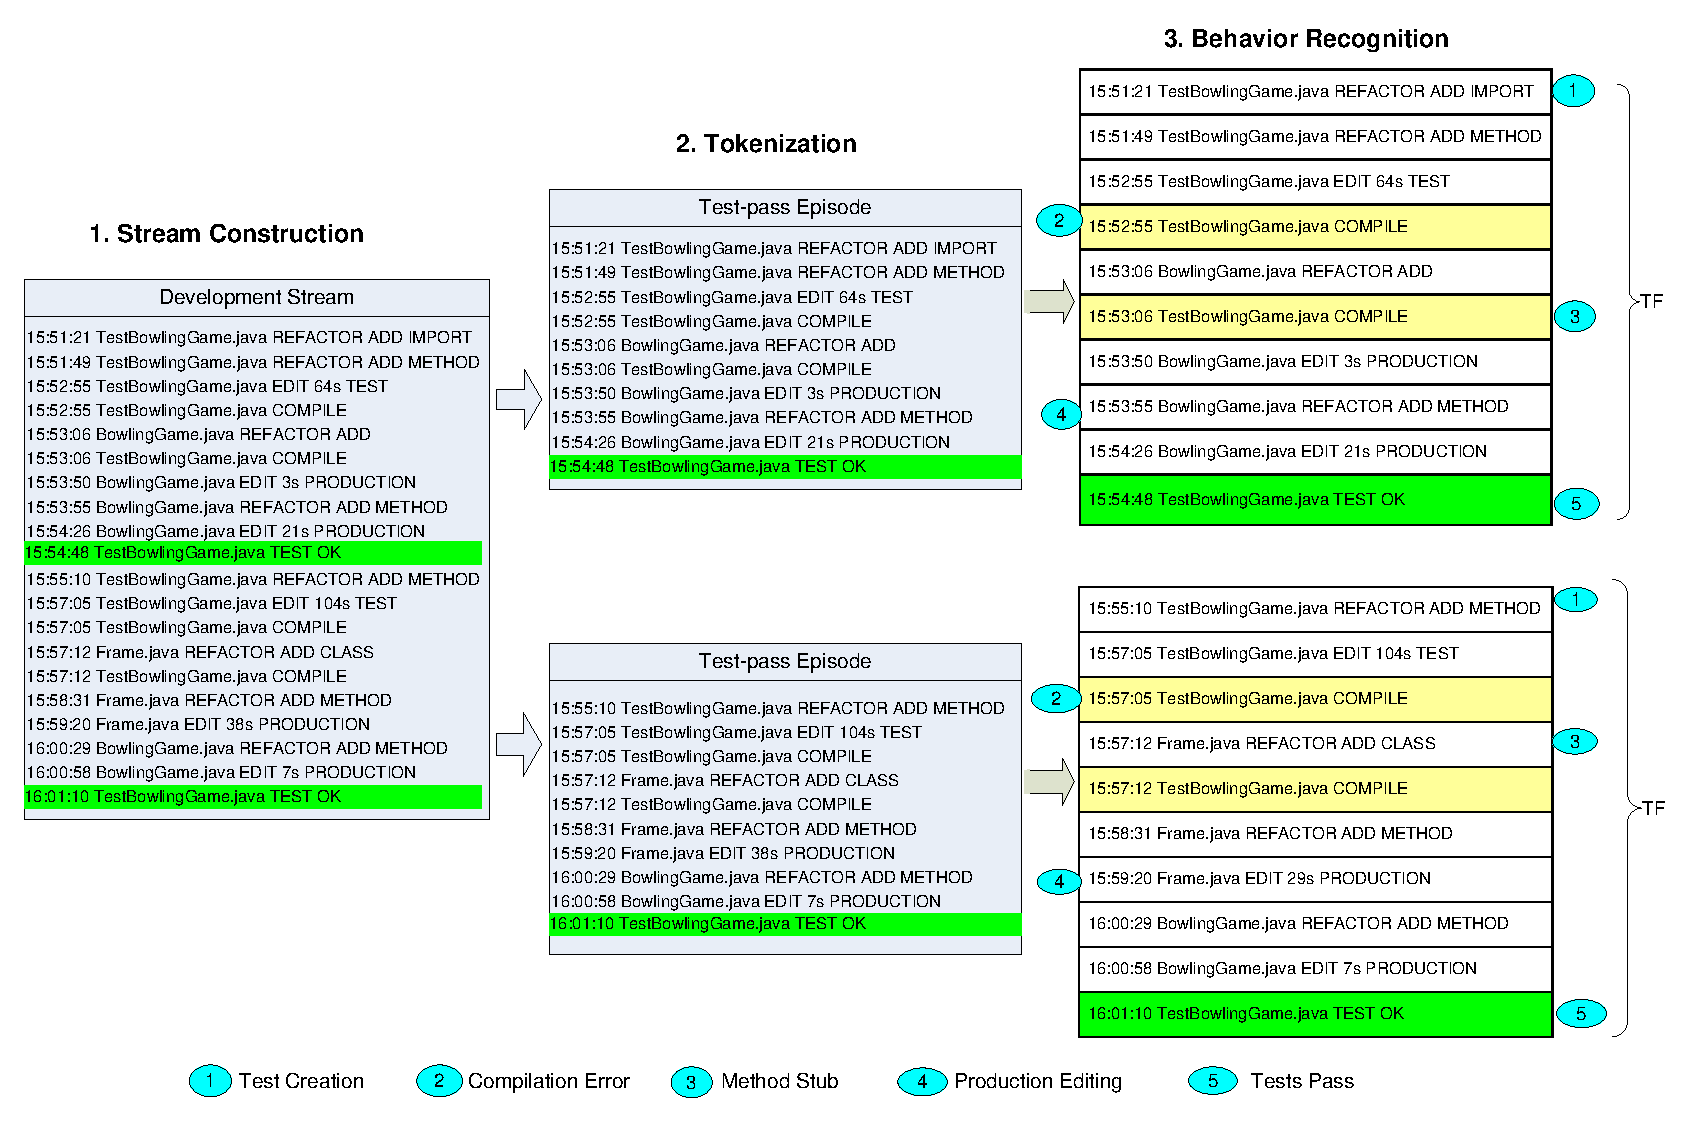
\includegraphics[width=1.0\textwidth]{Visio-SDSA-Example}
  \caption{Collecting, partitioning, and classifying developer behaviors}
  \label{fig:SDSA-Example}
\end{figure}

From 15:51:21 to 16:01:10, a developer implemented two user stories of the
bowling game in Test-Driven Development. We used Hackystat to instrument
the development process and collect sensor data regarding 
refactoring, editing, compilation and test invocation activities.  The ``Stream
Construction'' phase results in the consolidation of the raw Hackystat
sensor data into a sequence of 21 developer actions. Each action includes a
timestamp (such as 15:51:21), a file (such as ``TestBowlingGame.java''),
and an action type (such as ``EDIT 64s TEST'').

Among the 21 developer actions are two successful test invocation actions
(``TEST OK'').  Zorro partitions the stream of developer actions into
episodes based upon the occurrence of a successful test invocation action,
so this sequence of 21 actions is partitioned into two episodes, both
ending with a successful test invocation action.

The next step is to determine which, if any, of these two episodes
corresponds to a valid TDD development practice.  To do this, Zorro applies
a rule-based recognition system.  In this example, both episodes contain
the following sequence of actions: (a) a test method is created; (b) a
compilation error results; (c) a method stub is created in production code
which results in a successful compile; (d) more production code is edited;
and (e) all tests pass.  These actions correspond to the classic style of
TDD development, and Zorro's rules will classify both of these episodes as
instances of TDD.

Of course, in the case of simple toy examples where a developer follows the
canonical TDD approach, it is not surprising that Zorro can identify the
behavior as TDD.  The more important issue is how to deal with the
complexities of real world software development behaviors. 

\subsection{Episode Classification}

The heart of Zorro is its episode classification algorithm, implemented as
a set of JESS rules.  Figure \ref{fig:Categories} summarizes the effect of these rules, which is to classify any episode as belonging to one of 22 episode types. 

\begin{figure*}[th]
  \center
  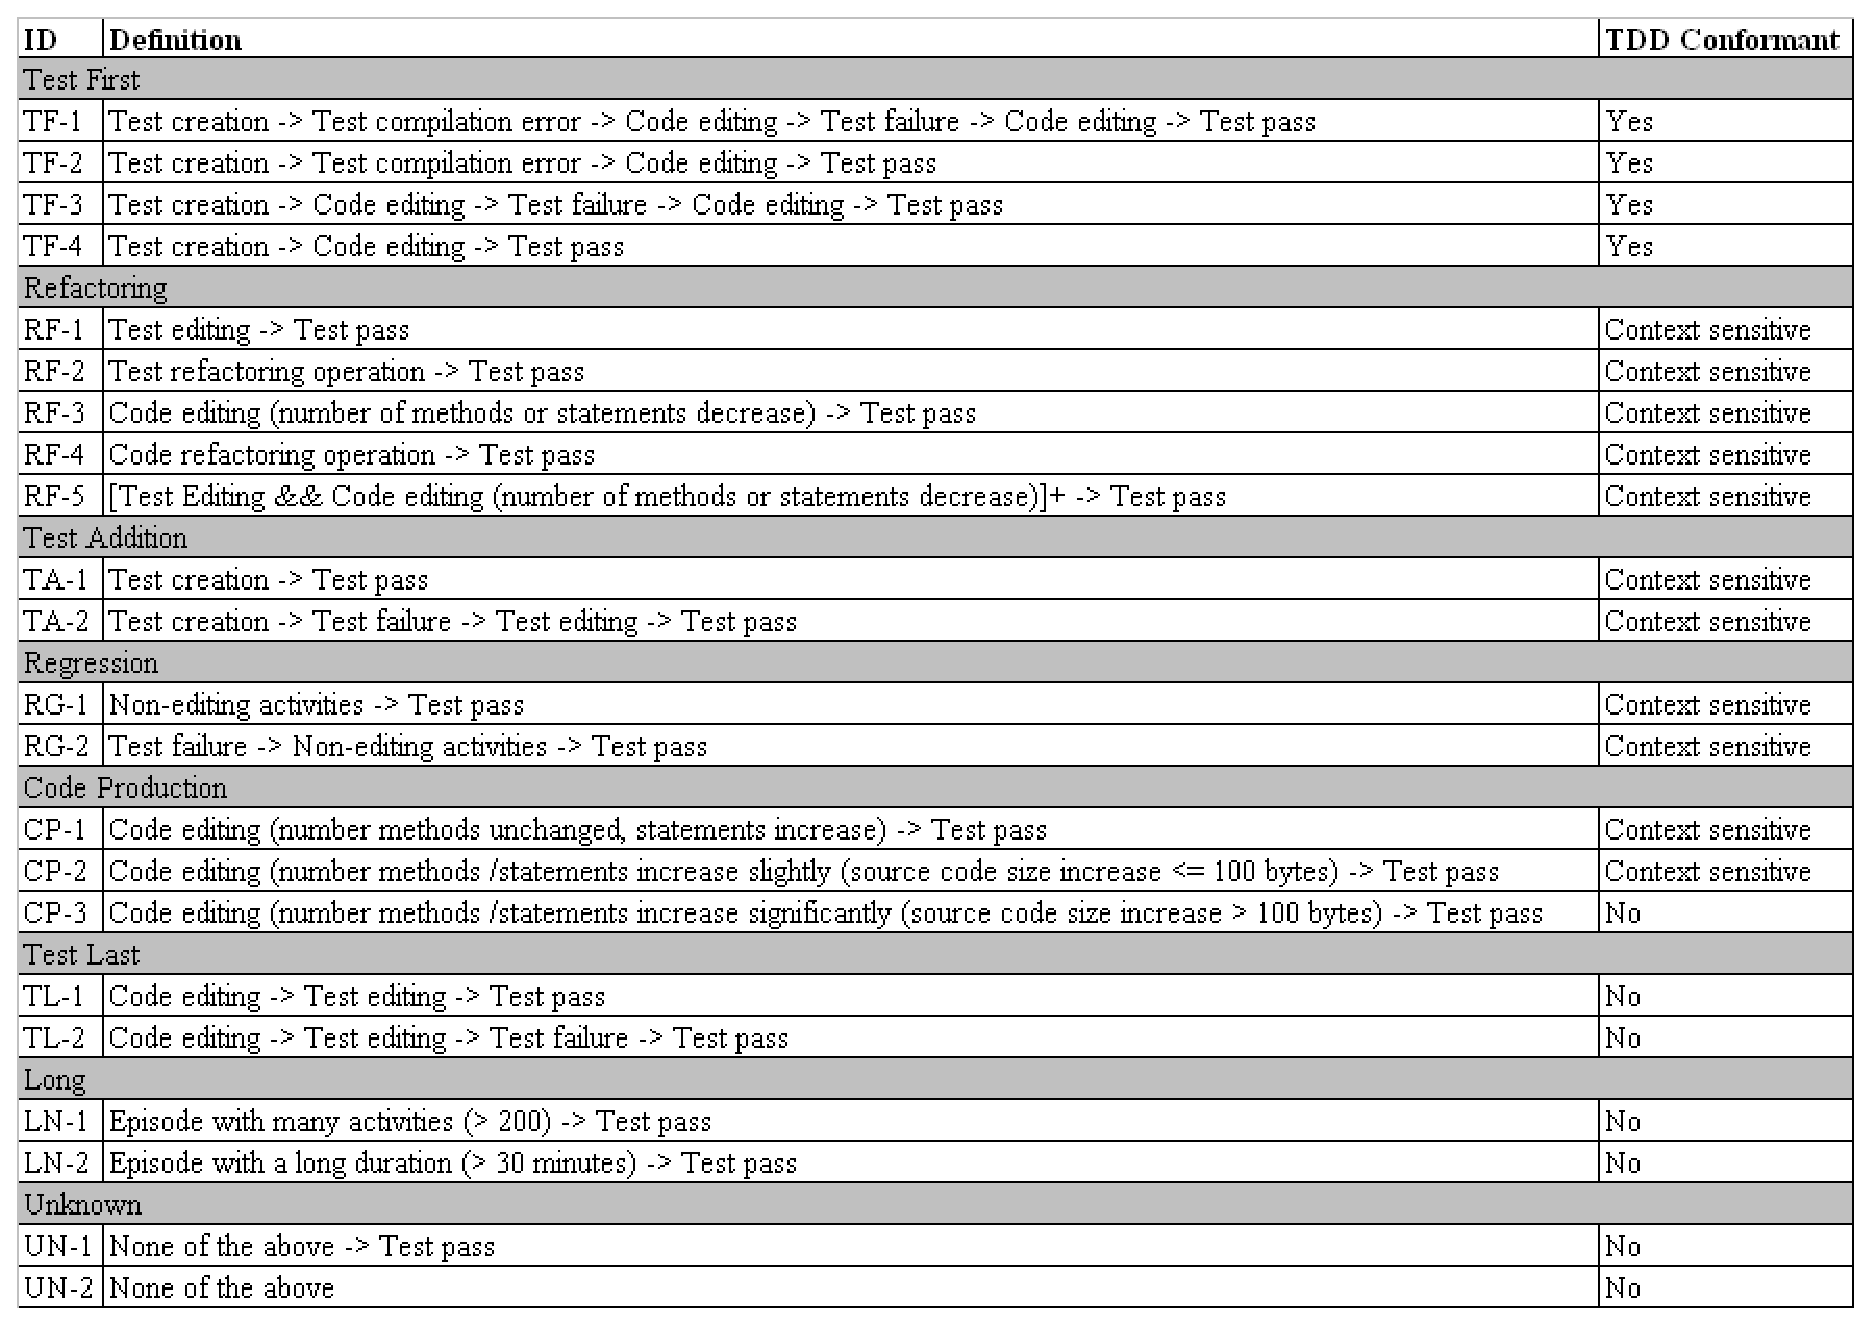
\includegraphics[width=1.0\textwidth]{episode-classification.eps}
  \caption{Zorro episode types, definitions, and TDD conformance}
  \label{fig:Categories}
\end{figure*} 

Zorro organizes the 22 episode types into eight categories: Test First
(TF), Refactoring (RF), Test Last (TL), Test Addition (TA), Regression
(RG), Code Production (CP), Long (LN), and Unknown (UN).  All of these
episode types (except UN-2) always ends with a ``Test pass'' event, since that
is the episode boundary condition.  (UN-2 is provided as a way to classify
a development session where there is no unit testing at all.)

Once each episode instance has been assigned an episode type by the SDSA
rule set, the final step in the Zorro classification process is to
determine the TDD conformance of that instance.  Figure
\ref{fig:Categories} shows that instances of some of the episode types are
easy to characterize. For example, every instance of a Test First episode
type is automatically TDD conformant, just every instance of a Test Last,
Long and Unknown episode type is automatically not TDD conformant.

Interestingly, several of the episode types, such as Refactoring, Test
Addition, Regression, and certain Code Productions are ambiguous: in
certain contexts, they could be TDD conformant, while in others they could
be TDD non-conformant.  This is because, for example, ``Refactoring'' can
legitimately occur while a developer is either doing Test Driven Design or
some different development approach, such as Test Last programming.  In
order to classify instances of these episode types, Zorro applies the
following heuristic: if a sequence of one or more ambiguous episodes are
bounded on both sides by non-TDD conformant episodes, then these ambigous
episodes types are classified as non-TDD conformant.

To make this clear, let's consider some examples, such as the episode
sequence [TF-1, RF-1, CP-1, TF-2].  In this sequence, Zorro classifies the
ambiguous episodes (RF-1 and CP-1) as TDD conformant, since they are
surrounded by TDD conformant episode types (TF-1 and TF-2).  Now consider
the sequence: [TL-1, RF-1, CP-1, TL-2].  In this sequence, Zorro classifies
the same two ambiguous episodes (RF-1 and CP-1) as TDD non-conformant,
since they are surrounded by non-TDD episode types (TL-1 and TL-2).

Now consider a sequence like: [TF-1, RF-1, CP-1, TL-1].  Here, the two
ambiguous episodes (RF-1 and CP-1) are surrounded on one side by an
unambiguously TDD conformant episode (TF-1) and on the other side by an
unambiguously TDD non-conformant episode (TL-1).  In this case, Zorro's
rules could implement an ``optimistic'' classification, and assign the
ambiguous episodes as TDD, or a ``pessimistic'' classification, and assign
the ambiguous episodes as non-TDD.  The current Zorro definition of TDD
implements an ``optimistic'' classification for this situation.

The Zorro classification system illustrates two important advances in our
approach to TDD.  First, it replaces the simplistic three episode type
(red, green, yellow) approach to TDD developer behavior with a more
sophisticated classification scheme based upon 22 distinct episode
types. Second, it reveals that the mapping from developer behaviors to TDD
is not straightforward. One can reasonably question whether the
``optimistic'' classification scheme currently chosen for Zorro is correct.
The resolution to this question, and indeed to questions regarding any
chosen operational definition of TDD, is {\em validation}: the process of
gathering evidence to determine whether the chosen definition matches
reasonable expectations for what constitutes TDD and what doesn't. We will
return to this issue in Section \ref{sec:validation}.


\subsection{Zorro Analyses}

Having collected the raw data using Hackystat sensors, and having
abstracted the raw data into episodes and classified it using SDSA, the
final step in Zorro is to provide analyses that are useful to both TDD
developers and TDD researchers.  This section overviews a few of the
analyses provided by Zorro to provide a flavor for what is possible with
this approach.

The first analysis, illustrated in Figure \ref{fig:Analysis-Table}, is
designed to provide visibility into the Zorro data collection and
classification process.

\begin{figure*}[th]
  \center
  \includegraphics[width=1.0\textwidth]{zorro-episode-interface.eps}
  \caption{Zorro Classification Analysis}
  \label{fig:Analysis-Table}
\end{figure*} 

Figure \ref{fig:Analysis-Table} displays two episodes, the first containing
19 development stream events and the second containing 10 development
stream events.  The display of each event includes its time-stamp, its
associated file (if applicable), and some additional information about the
associated sensor data.  The final column provides information about {\em
how} Zorro classified the episode (as either TDD conformant, or TDD
non-conformant), as well as {\em why} Zorro classified the episode that way
(via a textual summary of the episode structural characteristics used in
the classification).  

The analysis in Figure \ref{fig:Analysis-Table} is useful for those wishing
to understand Zorro's operational definition of TDD in the context of
actual development, either for learning or validation purposes.  Figure
\ref{fig:Analysis-Demography} provides a higher level perspective, by
showing only the sequence of episode types, with each TDD conformant
episode shaded in green. Clicking on an episode type drills down to a more
detailed description similar to that shown in Figure
\ref{fig:Analysis-Table}.

\begin{figure*}[th]
  \center
  \includegraphics[width=0.80\textwidth]{zorro-episode-demography.eps}
  \caption{Zorro Episode Demography}
  \label{fig:Analysis-Demography}
\end{figure*} 

Zorro provides a number of additional analyses that enable the developer to
understand the impact of TDD practices on their software product and
process.  Figure \ref{fig:Analysis-Ratio} shows how the ratio of test code
to non-test (production) code changes during the course of a development
session.  The horizontal bar at 1.0 represents equal amounts of test and
production code.  This figure illustrates a scenario of initial module
development in which there was significantly more production code than test
code at the beginning of the session, but the proportion of test code rose
until it doubled the amount of production code, before returning to 1.5
times the production code at the end of the session.

\begin{figure*}[th]
  \center
  \includegraphics[width=0.80\textwidth]{zorro-test-production-size-ratio.eps}
  \caption{Zorro Test/Production Size Ratio}
  \label{fig:Analysis-Ratio}
\end{figure*} 

The final example analysis illustrated in Figure
\ref{fig:Analysis-Telemetry} pops up to yet another level of abstraction by
using Software Project Telemetry, a capability of Hackystat that enables
the visualization of trends in process and product data over days, weeks,
or months.  In this real world data, two trends are displayed over the
course of eight weeks: the percentage of TDD conforming episodes, and the
test case coverage of the system under development.  Interestingly, the
level of test case coverage co-varies with the ``level'' of TDD practiced
by the developer.

\begin{figure*}[th]
  \center
  \includegraphics[width=0.80\textwidth]{zorro-tdd-coverage-2.eps}
  \caption{Zorro TDD Episode Telemetry}
  \label{fig:Analysis-Telemetry}
\end{figure*} 


\section{Validation}
\label{sec:validation}

In order to feel confident in Zorro as an appropriate tool to investigate
TDD, we must address two basic validation questions: (1) Does Zorro collect
the behaviors necessary to determine when TDD is occurring, and (2) Does
Zorro correctly recognize test-driven development when it is occurring?

The first validation issue addresses the use of automated, unobtrusive,
sensor-based data collection, and whether this approach can actually
acquire the data necessary to determine when TDD is taking place.

The second validation issue addresses our operational definition of TDD
based upon episode-based classification, and whether it provides a robust,
useful, and acceptable definition of TDD.

We began Zorro validation in the Spring of 2006 with a pilot study, and 
are building on that initial work in 2007.

\subsection{The pilot validation study}

To obtain some initial validation data on Zorro, we conducted a pilot study
in Spring of 2006 in which we instrumented the development environment with
Zorro sensors, asked a small set of students to do some simple TDD
development, then compared the resulting Zorro TDD classifications to an
independently collected source of data regarding their development
behaviors.

One approach to independent data collection would be to have an observer
watching the developers as they programmed, taking notes as to whether they
are performing TDD or not.  We considered this but discarded it as
unworkable: given the rapidity with which TDD cycles can occur, it would be
quite hard for an observer to notate all of the TDD-related events that can
occur literally within seconds of each other. We would end up having to
validate our validation technique!

Instead, we developed a plugin to Eclipse called the ``Eclipse
Screen Recorder'' (ESR).  This system generates a Quicktime movie
containing time-stamped screen shots of the Eclipse window at regular
intervals. One frame/second was found to be sufficient for validation,
generating file sizes of approximately 7-8 MB per hour of video.  The
Quicktime movie created by ESR provides a visual record of developer
behavior that can be manually compared to the Zorro analysis using the
timestamps and used to answer the two validation questions.

Our pilot validation study involved the following procedure. First, we
obtained agreement from seven volunteer student subjects to participate in
the pilot study. These subjects were experienced with both Java development
and the Eclipse IDE, but not necessarily with test-driven development.
Second, we provided them with a short description of test-driven design,
and a sample problem to implement in a test-driven design style.  The
problem was to develop a Stack abstract data type using test-driven design,
and we supplied them with an ordered list of tests to write and some sample
test methods to get them started.  Finally, they carried out the task using
Eclipse with both ESR and Zorro data collection enabled.

To analyze the data, we created a spreadsheet in which we recorded the
results of watching the Quicktime movie and manually encoding the developer
activities that occurred.  Then, we ran the Zorro analyses, added their
results to the spreadsheet, and validated the Zorro classifications against
our analysis of the video record.

The participants spent between 28 and 66 minutes to complete the task.
Zorro partitioned the overall development effort into 92 distinct episodes,
out of which 86 were classified as either Test-Driven, Refactoring, or
Test-Last; the remainder were ``unclassified'', which normally corresponded
to startup or shutdown activities.  Note that the version of Zorro used in
Spring 2006 used a somewhat less sophisticated classification ruleset than
the current version.

Out of the 92 episodes under study, 82 were validated as correctly
classified, for an accuracy rate of 89\%.

\subsection{Ongoing validation}

The pilot study provided us with valuable feedback about the potential
utility of Zorro, as well as deeper insight into the process of validation
itself.  Our current research is focused on enhancing our understanding of
the strengths and weaknesses of Zorro with several additional validation
studies.

Our next validation study will also involve students, and will expand on
the pilot study by cross-validating the Zorro operational definition of TDD
against two independent data sources: the ESR video stream and the feedback
of the participants themselves following the TDD development session.  We
will ask them to review the TDD episodes generated by Zorro and provide
their personal feedback on the classifications.

Following this second student-based validation study, we plan to gain
insight into the strengths and weaknesses of Zorro in professional
settings.  For this case study, we will invite developers who
practice TDD and who use Eclipse, Java, and JUnit to help us validate
Zorro.  The process involves installing the Hackystat Eclipse sensor for
Zorro into their development environment, performing development for a few
days with the sensors installed, then reviewing the classifications made by
Zorro and providing us with feedback regarding its accuracy.

We also plan to obtain feedback from the TDD research community.  We believe
that Zorro can provide useful infrastructure for research on test driven
development.  For this case study, we will invite researchers to 
evaluate Zorro against their experimental requirements and provide us with 
feedback as to the suitability of Zorro for their own work. 

\section{Contributions and future directions}
\label{sec:conclusions}

This research contributes in the following ways to the research and
practice of test-driven development in particular, and automated software
engineering in general.

First, to our knowledge, Zorro is the first, and so far only,
fully-automated system capable of recognizing test-driven development
practices.  As we noted above, such a system can address the 
process compliance problem from which much current TDD research suffers. 

Second, by providing fully automated recognition, Zorro provides the first
precise, operational definition of TDD practice.  Our research revealed
that this operational definition was not straightforward to implement, as
certain kinds of episode typeswere intrinsicially ambiguous.  Resolving
these episode types required the implementation of disambiguation
heuristics. Our empirical evaluations demonstrated that these heuristics
seemed satisfactory in most situations.

Third, this research results in a new approach to measuring TDD compliance
based upon ``episodes'', or short-duration intervals of development.  Using
Zorro, one can speak of a development team as having used TDD ``55\% of the
time during the previous week''.  This much more fine-grained
characterization enables new kinds of research on TDD, such as whether
there is a threshold for TDD use.  For example, perhaps productivity and
quality do climb with TDD use up to a threshold of, say, 80\%, beyond which
there is no discernable improvement.  As another example, perhaps there is
a steep drop-off in quality and/or productivity if TDD usage drops below,
say, 30\%.

Finally, the Zorro system was implemented within the Software Development
Stream Analysis (SDSA) framework.  SDSA provides a generic means for
recognition of developer ``micro-processes'' such as TDD.  In future work,
we hope to write new applications on top of SDSA in addition to Zorro, such
as an application for recognizing Continuous Integration best practices.

\begin{acknowledgements}
We gratefully acknowledge the members of the Collaborative Software Development Laboratory (etc.).
\end{acknowledgements}

\bibliographystyle{spbasic}      % basic style, author-year citations
% The \cite command functions as follows:
 %   \citet{key} ==>>                Jones et al. (1990)
 %   \citet*{key} ==>>               Jones, Baker, and Smith (1990)
 %   \citep{key} ==>>                (Jones et al., 1990)
 %   \citep*{key} ==>>               (Jones, Baker, and Smith, 1990)
 %   \citep[chap. 2]{key} ==>>       (Jones et al., 1990, chap. 2)
 %   \citep[e.g.][]{key} ==>>        (e.g. Jones et al., 1990)
 %   \citep[e.g.][p. 32]{key} ==>>   (e.g. Jones et al., p. 32)
 %   \citeauthor{key} ==>>           Jones et al.
 %   \citeauthor*{key} ==>>          Jones, Baker, and Smith
 %   \citeyear{key} ==>>             1990
\bibliography{tdd,zorro,csdl-trs,hackystat,psp}
\end{document}


% So far, software engineering researchers have focused most of their 
% energy on the outcomes that applying TDD brings to software products 
% and software developers. However, compared to the claims made by 
% practitioners, research findings of TDD on software quality and 
% developer productivity are mixed. In fact, much of the research work on TDD 
% suffers from the threat of ``construct validity'' \cite{Wang:04} 
% because of the ``process conformance'' problem. Wang and Erdogmus define 
% process conformance as ``the ability and willingness of subjects to follow 
% a prescribed process''. Janzen and Saiedian warn that the inability to 
% accurately characterize process conformance is harmful to TDD research, 
% and that it is so hard to measure the usage of a development method 
% such as TDD that current reports on adoption of TDD are not valid. 
% Surveys are often used to measure the adoption of TDD, but only those 
% who are much in favor or much opposed to it will respond. Janzen and 
% Saiedian concluded that the combination of popularity of XP, JUnit 
% and Eclipse likely implies a certain degree of adoption of TDD 
% \cite{Janzen:05}. However, this is a very indirect measure.

% Some of research work 
% \cite{Cook:95,Jensen:05,csdl2-06-02,Wang:04,Wege:04} has been 
% done on software process compliance using development activities 
% and software artifacts collected from the development process. 
% In my dissertation research, I focus on studying the process 
% conformance of low-level software processes and Test-Driven 
% Development in particular. 

% Janzen claimed that TDD is a kind of software development method,
% not a process model, and that it has emerged out of a particular 
% set of process models \cite{Janzen:05}. In contrast, Beck and 
% Cunningham, the pioneers of TDD, put it this way: ``test-first 
% coding is not a testing technique but is rather about design.''
% \cite{Beck:01} If TDD is a design technique and it drives the 
% implementation of product code, then classifying it as a software 
% process sounds reasonable. In my research, I have characterized
% practices such as Test-Driven Development and Personal Software 
% Process (PSP) as low-level software processes. A common 
% characteristic of low-level software processes is that they are defined 
% by many frequent and rapid short-duration activities. Unlike high-level 
% and long duration phases such as ``requirement analysis'' that might 
% last weeks to months, the activities in low-level software process 
% such as ``refactor class Foo to extract interface IFoo'' may take 
% only seconds to a few minutes \cite{csdl2-06-02}.

% This chapter begins with a detailed introduction to TDD, followed 
% by a discussion of TDD empirical studies.
% The research results are mixed because of differences in experiment
% settings, and the empirical studies suffer from construct validity
% because of the process conformance problem of TDD. In the second
% part, I present other related work on automated process conformance 
% in contrast to my research that is built on the automated software 
% metrics collection machinery of 
% Hackystat \cite{Hackystat,csdl2-01-12,csdl2-01-13,csdl2-02-07}. 


%% In the next section, we examine some of the issues that could influence these findings. 

%% \subsubsection{Issue: Students vs. Professional Developers}

%% One difference is in population. The studies in academic settings (noted by
%% an ``A'' in the ``A/I'' column) used students as test subjects, while the
%% studies in industrial settings (noted by an ``I'' in the ``A/I'' column)
%% recruited professional developers.  Of 10 empirical studies listed in the
%% two tables, 5 were conducted in academic settings, and the other 5 were
%% conducted in industrial settings. The studies conducted in industrial
%% settings found evidence of software quality improvements, but often at the
%% cost of decreased developer productivity. On the contrary, the studies in
%% academic settings often found no software quality improvement but an
%% increase of developer productivity.

%% \cite{Maximilien:03} proposed TDD as a solution to reduce the defect
%% rate. \cite{Williams:03} assigned a dedicated coach to the development
%% team. \cite{George:03} noticed that the control group did not write
%% worthwhile automated tests, partially due to the lack of
%% incentives. \cite{Brilliant:99} note that industry does not perceive a
%% significant benefit from working with academic researchers in many
%% cases. Researchers have to be able to convince industry practitioners of
%% the benefits and provide assistance in order to conduct research in
%% industrial settings.  The benefits are important to the participants of
%% industrial studies, otherwise the quality of research would
%% degrade. \cite{Geras:04} reported that professional developers are hard to
%% recruit when participation is voluntary.

%% Students are generally less experienced at software development when
%% compared to professional software developers. It is unclear whether
%% students are appropriate participants for effectively studying TDD
%% \citep{Erdogmus:05}.  \cite{Muller:02} reported that the TDD group produced
%% code with 74\% branch converage only, while the control group produced code
%% with 80\% branch coverage.  \cite{Erdogmus:05} discussed the causal
%% relationship between research findings and participant skill levels. They
%% found that the students with high skill rate improved productivity more
%% dramatically than the students with low skill rate.

%% \subsubsection{Issue: Case Study vs. Controlled Experiment}

%% Another difference between the academic and industry based research is in
%% research methods. Case study and controlled experiment are the two most
%% popular research methods.  Of the 10 studies listed in the two tables, 6
%% are controlled experiments and 4 are case studies. Most of the controlled
%% experiments were conducted in academic settings because classroom settings
%% are more amenable to controlled experimentation.  Since industry rarely
%% repeats the same project twice, it is hard to have controlled experiments
%% in industrial settings. Two out of four of the industrial studies were case
%% studies.

%% In controlled experiments, researchers often isolated test first from TDD
%% to compare it against other development methods such as test last and
%% ad-hoc \citep{Muller:02,Matjaz:03, Erdogmus:05,George:03,Geras:04}. Half of
%% the controlled experiments \citep{George:03,Kaufmann:03,Erdogmus:05}
%% observed productivity improvement in TDD groups, but only two studies found
%% evidence of software quality improvement. On the contrary, the participants
%% in the case studies improved software quality dramatically after adopting
%% TDD, but they also spent more time on development.

%% \subsubsection{Issue: Choice of baseline development method}

%% A third difference among the studies is the choice of development methods
%% that TDD was compared against. Researchers compared TDD against the
%% traditional test-last \citep{Kaufmann:03,Geras:04}, ad hoc
%% \citep{Muller:02,George:03}, and iterative test last (ITL)
%% \citep{Matjaz:03,Erdogmus:05} methods. TDD did not help to improve software
%% quality when it was compared against ITL.  But it helped to improve
%% software quality when it was compared with ad hoc and test last
%% methods. Though TDD developers spent more development time, they also wrote
%% more tests \citep{George:03,Erdogmus:05} and ran tests more frequently
%% \citep{Geras:04}.

%% \subsubsection{Issue: Process conformance}

%% \cite{Erdogmus:05} explicitly addressed ``process conformance'' as a threat
%% to validity.  In order to improve process conformance, they informed
%% participants of the importance of following the proper procedures, and
%% conducted a post test survey to filter unconformant data points. Although
%% they first identified process conformance as a threat to the validity of
%% research results of TDD, they were not alone in dealing with it.

%% \cite{Muller:02} also indicated that their experiment was not technically
%% controlled.  During the experiment, they had to ask TDD groups if they were
%% following the test-first process.  \cite{Matjaz:03} instrumented Eclipse,
%% the development tool used in their study, to report unit test invocation
%% frequency, results and time taken. A similar instrumentation method was
%% used by \cite{Geras:04}. However, instrumenting test invocation is a poor
%% measure for process conformance of TDD because developers in test last
%% groups can also run tests frequently. In
%% \citep{George:03,Williams:03,Maximilien:03}, researchers studied test-first
%% along with pair programming, which served as the process control
%% method. Clearly, none of these methods is reliable at controlling
%% participants' compliance to TDD as opposed to alternative development methods.
